\section{Equivalence of RTL and Software Netlist}~\label{sec:props}
%
The consistency between two designs can be established in several ways. 
For example, a few common notions of consistency are \emph{behavioral}, 
\emph{cycle-accurate}, \emph{non-cycle accurate} or \emph{functional}
consistency.  The consistency between a reference model and an implementation
model is established through systematic equivalence 
checking~\cite{CKY03,DBLP:conf/date/KoelblJJP09,DBLP:journals/tcad/StoffelK04,
DBLP:conf/date/Eijk98,DBLP:conf/iccd/BaumgartnerMPKJ06}.  Equivalence checking between a timed and untimed model is a hard
problem~\cite{kuehlmann2002combinational}.  Sequential equivalence checking techniques 
are used to check the equivalence between an asynchronous event driven semantics of C and synchronous 
clock driven semantics of Verilog~\cite{CKY03, DBLP:conf/iccd/BaumgartnerMPKJ06}.


%%%%%%%%%%%%%%%%%% CYCLE ACCURATE EQUIVALENCE %%%%%%%%%%%%%%%%%
Two designs are said to be \emph{cycle-accurate-equivalent}~\cite{cycle,kuehlmann2002combinational} 
if they produce the same output using the same number of clock cycles.   
%%%%%%%%%%%%%%%%%% NON-CYCLE ACCURATE EQUIVALENCE %%%%%%%%%%%%%%%%%
On the other hand, two designs are \emph{not} cycle-accurate-equivalent if they require 
different cycles to perform the same computation. For example, consider two circuits
implementing Euclid's algorithm to compute Greatest Common Divisor (GCD),
where Circuit A uses two subtractors and Circuit B uses one subtractor. Assume that 
Circuit B requires more cycles than Circuit A for computing the GCD. Thus,
they are functional-equivalent but not cycle-accurate-equivalent. However,
Circuit A and Circuit B can be made cycle-accurate-equivalent by making Circuit
A to stutter for few cycles until Circuit B finishes its slower operation.  This
may require some additional logic in Circuit A to determine the condition for 
stuttering.  


In this paper, we consider the equivalence between the RTL circuits and the 
software netlists that preserve the following - 1) the input-output behavior, and 
2) the outcome of all assertions (temporal or non-temporal) must match in the RTL 
as well as in the software netlist design.  
% 
We first present the property specification language and then define the 
property-based observable equivalence. 
% 
\subsection{Properties}~\label{properties}
%
System Verilog Assertions (SVA) property specification language is most commonly used 
to write properties of RTL designs.  The SVA properties can be translated 
into an intemediate Linear Temporal Logic (LTL)~\cite{DBLP:journals/jacm/SistlaC85} 
representation.  LTL is a modal logic that is commonly used to reason about a hardware 
transition system.  The modalities in LTL refer to
temporal operators such as $G$ (global), $F$ (eventual), $X$ (next) and $U$
(until).  An LTL formula may contain propositional symbols, boolean or temporal
operators.  We refer the reader to~\cite{DBLP:journals/jacm/SistlaC85,mc-book} 
for more details on LTL. 


The translation of LTL to a \emph{Buchi Automaton}
(BA) is a well-known technique~\cite{Gastin:2001, SomenziB00} and has been
successfully used for LTL model checking, such as the Spin model checker~\cite{spin}.   
Further, a Buchi Automaton can be modeled using a C program that simply encodes
its state transition relation.  
%
In this paper, we use System Verilog Assertions (SVA) to express properties of 
the RTL designs. The SVA properties are translated into equivalent C assertions 
either using \emph{v2c} or manually.  An alternative option, which we did not explore 
in this work, is to construct a property compiler for automatically translating the 
SVA properties to assertions in C language. 
%
\Omit{
The translation of purely propositional properties is straightforward.  While, 
the translation of temporal properties are done following the notion of equivalence 
described in Section~\ref{eq-sw-hw}. 
}
%

Figure~\ref{fig:prop} gives an example of SVA, its equivalent LTL, 
and the corresponding assertion in the software netlist for the 
design of Figure~\ref{figure:equivalence}.
%
The next time operator $X$ in LTL is 
modeled by invoking the top-level procedure
$M(clk,in,out1,out2,out3)$ in the software netlist. 
Note that the top-level procedure in the software netlist 
corresponds to the top-level module of the RTL design.  
%
\Omit{
The granularity 
of the effect of one clock step is modeled by invoking 
the top-level procedure in the software netlist.
}
%
\begin{figure}[t]
\scriptsize  
\centering
\begin{tabular}{|l|l|}
\hline
 Buchi Automaton & Assertion in $\mathcal{SN}$ \\
\hline
\begin{minipage}{3.5cm}
\scalebox{.5}{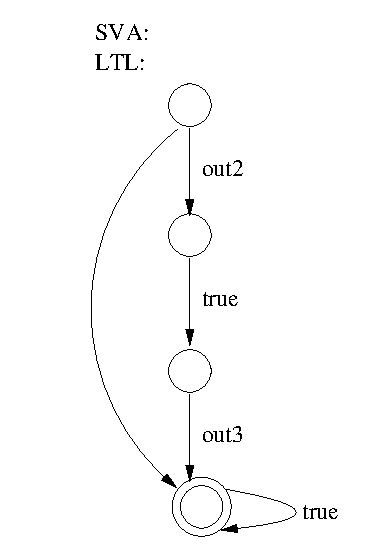
\includegraphics{figures/property_pspdftex.eps}}
\end{minipage}
&
\begin{lstlisting}[mathescape=true,language=C]
if(sM.out2) {
  M(clk,in,out1,out2,out3);
  assert(sM.out3);
}
\end{lstlisting}
\\
\hline
\end{tabular}
\caption{LTL and its corresponding C assertion}
\label{fig:prop}
\end{figure}
%
%The goal of this translation is to perform formal property verification 
%of the software netlist against the assertions given in SVA.
%expressed over the variables of $\mathcal{SN}$.  
%
%%%%%%%%%%%%%%%%%% RESTRICTED CYCLE ACCURATE EQUIVALENCE %%%%%%%%%%%%%%%%%
\subsection{Property-based Observable Equivalence}
%
Recall that a RTL design in Verilog is translated into a software 
netlist in C for the purposes of formal verification.  To this end, the formal specification or 
properties (temporal or non-temporal) over RTL signals that capture 
hardware behaviors are translated into assertions over the 
corresponding software variables in the software netlist and 
checked for consistency against the software netlist. 
Thus, our notion of equivalence is based on the signals 
that are observable in the properties under consideration. 
We call this equivalence criteria 
\emph{property-based observable equivalence}. 
Intuitively, this means that the state of latches and wires 
referred to by the property must match with the corresponding 
variables in the software netlist at some designated clock cycle.  
% 
Let us consider the temporal assertion given by, \texttt{a |-> \#\#4 b}.  
Formal verification tools for hardware unwinds the RTL transition 
system~4 times for checking the property. Here, unwinding means duplicating the 
transition system~4 times. Similarly, the software netlist is also unwound~4 times 
for checking the property. Hence, the simulation of the RTL clock is achieved by 
unwinding the transition system of the software netlist design. 
% 
By means of experiment, we show that for designs considered in this 
paper, that is, for single-clock designs without clock-gating 
or power-gating, abstracting the RTL clock in the software netlist 
does not have any impact on the verification outcome. However, designs that 
exhibit clock-gating or power-gating techniques~\cite{lowpower} or 
designs that contain multiple clocks may be non-trivial to translate into the 
software netlist and may require modeling the behavior of clock explicitly.
% 
%%%%%%%
\Omit{
Recall that the effect of a clock cycle in the software netlist 
is simulated through an invocation of the top level procedure 
which corresponds to the top level module of the RTL~\cite{mtk2016}.  
} 
% 
%
\Omit{Note that a software netlist is synthesized from a hardware
RTL for the purposes of formal verification, just like a bit-level netlist or
word-level netlist are synthesized from an RTL. So, the proposed consistency 
criteria is sufficient for this purpose.}  
%
\begin{definition}~\label{verilog-c-eq} (Property-based Observable Equivalent) 
  Two designs $C_1$ and $C_2$ are \emph{property-based observable equivalent} with
  respect to a property $P$ if the following conditions hold.  Note that we assume 
  that the verification outcome of these properties are obtained using the native 
  verifiers for software and hardware.  The verification outcome can be 
  either \emph{safe} in which case $P$ holds on $C_1$ and $C_2$, or \emph{unsafe} 
  in which case $P$ does not hold on $C_1$ nor on $C_2$. 
  \begin{enumerate}
    \item For a non-temporal property $P$, the verification outcome of $P$ must
      match in $C1$ and $C2$ at every clock cycle.  
   \item For a temporal property $P$, the verification outcome of $P$ must 
     match in $C_1$ and $C_2$ at clock cycles determined by the temporal 
     operator used in $P$.  We explain this below.  
     %some \emph{designated} clock cycle.  Such designated clock cycle 
     %is determined by the temporal operator used in $P$. 
  \end{enumerate}
\end{definition}
%
Two designs $C_1$ and $C_2$ are \emph{not} property-based observable equivalent 
with respect to a non-temporal property $P$ if there exist a clock cycle where 
the verification outcomes of $P$ in $C_1$ and $C_2$ do not match.  Intuitively, 
this means that at some cycle $N$, 
%there exists some latches or wires 
the state of latches or wires that are referred to by $P$, does not match in 
$C_1$ and $C_2$, resulting in inconsistent verification outcome for $P$. 
% 
On the other hand, two designs $C_1$ and $C_2$ are \emph{not} property-based observable equivalent 
with respect to a temporal property $P$ if there exists a \emph{designated} clock cycle 
where the verification outcomes of $P$ in $C_1$ and $C_2$ do not match.  



%%%%%%%%%%%%%%%%%% EXAMPLE %%%%%%%%%%%%%%%%%
\begin{example}
%
Figure~\ref{figure:equivalence} gives an example of a Verilog RTL design 
(on the left) and the corresponding software netlist in C (on the right) that are 
property-based observable equivalent with respect to a temporal 
property (marked in blue).  The property in the Verilog RTL design 
is specified in SystemVerilog Assertion (SVA)~\cite{SVA} language.  
The equivalent assertion in the software netlist is shown on the right (marked in blue).  


Figure~\ref{fig:waveform} gives the waveform view that shows the behavior 
of the RTL design of Figure~\ref{figure:equivalence}. 
% 
We explain the equivalance of the Verilog RTL and the 
software netlist design with respect to the temporal SVA 
assertion given by \texttt{(in==1 |-> \#\#1 out3)}.  
%


Suppose \texttt{in=1} at clock cycle $i$.  Then, the state of 
the latch \texttt{out3} is not consistent in Verilog and C at 
cycle $i$.  This is due to the fact that 
the value of \texttt{out3} \emph{stabilizes} one cycle after the 
input \texttt{in=1} was set, that is, \texttt{out3} is stabilized in cycle $i+1$.  
This behavior is formally captured 
in SVA by the expression \texttt{(in==1 |-> \#\#1 out3)}.  
The SVA property specifies that the latch \texttt{out3} is high 
exactly one cycle after \texttt{in} was high.  
%

Recall from Definition~\ref{verilog-c-eq} that for two designs to be 
property-based observable equivalent with respect to the temporal 
property $P$,  the verification outcome of $P$ must match in the 
two designs at some designated clock cycle. 
% 
For the above SVA assertion, the designated clock cycle is specified 
by \texttt{\#\#1} delay operator.  That is, the value of \texttt{out3} 
must match in Verilog and the software netlist one cycle after the 
event $\texttt{(in==1)}$ has occured. 
% 
Thus, the value of \texttt{out3} may be inconsistent in Verilog and software netlist 
in clock cycle $i$ when the event $\texttt{(in==1)}$ has occured, but 
the property still holds in both the designs since the output value of 
\texttt{out3} matches in clock cycle $i+1$. 
% 
We use a state-of-the-art hardware model checker and a commercial 
software analyzer to verify the RTL and the software netlist respectively.  
The above SVA property is proven equivalent for an unbounded number of cycles in 
both the designs.  Hence, both the designs are property-based observable equivalent.
\end{example}
% 
\begin{figure}[t]
\centering
\scriptsize
\begin{tabular}{l|l}
\hline
Verilog RTL & Software netlist (in C) \\
\hline
\begin{lstlisting}[mathescape=true,language=Verilog,style=base]
module M(clk, in, 
     out1, out2, out3);
input clk,in;
output reg out1, 
     out2, out3;
wire t1;

initial begin
out1=0; 
out2=0;out3=0;
end

assign t1=out1;

always @(in) begin
out1 <= in;
end

always@(t1) begin
out2 <= t1;
end

always@(posedge clk) 
begin
out3 <= out2;
end
endmodule

module main(clk);
input clk;
wire in,out1,
     out2,out3;
M m1(clk,in,out1,out2,out3);
~assert property ~
 ~(in |-> ##1 out3);~
endmodule
\end{lstlisting}
&
\begin{lstlisting}[mathescape=true,language=C,style=base]
struct state_M {
 bool out1, out2, out3; 
};
struct state_M sM;

void initial() {
 sM.out1=0; sM.out2=0; 
 sM.out3=0;
}

void M(bool clk, bool in, 
 bool *out1, bool *out2, 
 bool *out3) {
  bool t1;
  sM.out1=in;
  t1=sM.out1;
  sM.out2=t1;
  sM.out3=sM.out2;
  // update output  
  *out1=sM.out1;
  *out2=sM.out3;
  *out3=sM.out3;
}
 
int main()
{
 bool clk,in,
 out1,out2,out3;
 initial();
 ~while(1) {~
  ~if(in) {~
   ~M(clk,in,~
   ~&out1,&out2,&out3);~
   ~assert(sM.out3);~
  ~}~
 ~}~
}
\end{lstlisting}
\\
\hline
\end{tabular}
\caption{Property-based observable equivalence of RTL and Software netlist}
\label{figure:equivalence}
\end{figure}
%
\begin{figure}[t]
\begin{center}
  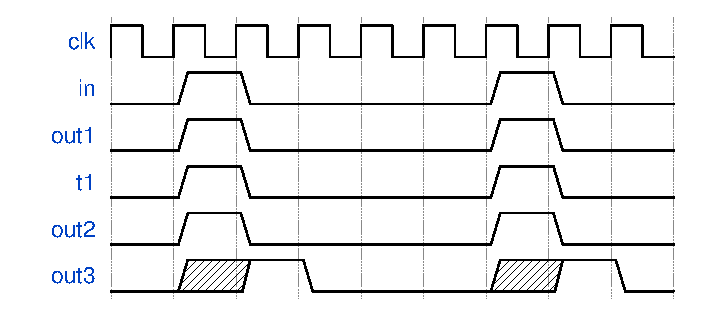
\includegraphics[width=\columnwidth]{figures/wavedrom.eps}%
  \caption{Waveform view showing behavior of RTL design in
  Figure~\ref{figure:equivalence}} 
\label{fig:waveform}
\end{center}
\end{figure}
%
Techniques such as translation validation~\cite{DBLP:conf/tacas/PnueliSS98}  
that check the consistency between an RTL and software is a different problem 
and beyond the scope of this work.
%
%While we do not have a formal proof of equivalence between the Verilog RTL and the 
However, experiments have shown that for 
property verification, valid safety properties are proven to be $k$-inductive for 
the same unwind depth $k$ in the RTL and the software netlist design.  Conversely, 
for unsafe designs, a bug is found in the same unwind depth for both the designs.
